% !Mode:: "TeX:UTF-8"
%!TEX program  = xelatex

\documentclass{cumcmthesis}
%\documentclass[withoutpreface,bwprint]{cumcmthesis} %去掉封面与编号页
\usepackage{caption}
\usepackage{url}
\title{高压油管的压力控制及方案设计}
\tihao{A}
\baominghao{201909044022}
\schoolname{上海科技大学}
\membera{胡珈瑜}
\memberb{肖涵薄}
\memberc{张婧萱}
\supervisor{}
\yearinput{2019}
\monthinput{09}
\dayinput{15}
\renewcommand\d{\mathop{}\!\mathrm{d}}
\newcommand{\f}[2]{\frac{#1}{#2}} 
\newcommand{\ar}[1]{
        \begin{aligned}                              %begin an array
            #1
        \end{aligned}   }  
\newcommand{\x}{&=}
\newcommand{\hua}[1]{\left\{\begin{aligned}
    #1
    \end{aligned}\right.}

\begin{document}

 \maketitle
 \begin{abstract}
问题旨在通过


\keywords{折叠桌\quad  曲线拟合\quad   非线性优化模型\quad  受力分析}
\end{abstract}

%目录
\tableofcontents

\newpage

\section{问题重述}
\subsection{背景介绍}
提高功率、节约能源与改善排放已经成为当今燃油机发展的必然趋势。为了与高性能燃油机相配合,必然要求高压燃油系统也具有极高的性能。

高压油泵、高压油管与喷射嘴是高压燃油系统中最为重要的组成部分。燃油进入与喷出的间歇性工作过程会导致高压油管内压力的变化,并使得喷油量出现偏差,这些偏差会影响发动机的工作效率。通过对高压油泵与喷油嘴等开关的控制,可以有效地维持高压油管内的压力从而保证喷油量的稳定,提高发动机的工作效率。

\subsection{具体问题}

(1)已知高压油泵压力及其单向阀休息时长、喷油器的工作状态、高压油管尺寸以及压力的变化要求,确定高压油泵单向阀的单次开启时长,使得油管内的压力波动尽可能较小。

(2)结合实际情况分析,将问题一中的恒压高压轴泵换为由凸轮驱动的柱塞,喷油嘴则由针阀周期性控制,其他条件均与第一题相同。在此基础上,确定凸轮的角速度,使得高压油管内的压力尽量稳定在100 MPa。

(3)在问题二的基础上,增加了一个喷油规律相同的喷油嘴与单向减压阀,使得管内的燃油可以回流到外部的低压油路中,进一步减小压力,从而给出更优化的高压油泵与减压阀控制方案。

\section{问题的分析}
\subsection{问题的总分析}
本题通过泵入, 喷出和回流来改变高压油管内的压强, 要求通过改变泵入和回流的油量来保持压强稳定。
本文的基本思路为通过计算机模拟,获得在不同条件下使得高压燃油系统保持稳定的最优控制方案。

\subsection{问题一的分析}
第一问是在压力差恒定的匀速泵油条件下,获得高压油管内压强尽可能稳定在100 MPa的单向阀最佳单次开启时长,本小题1 s内喷油量是已知的。 由于油管内压强始终在100 MPa上下浮动, 可以忽略每次泵油后由于高压油管内压力改变导致的泵油速率改变。 问题变为寻找合适的高压油泵单向阀开启时长, 使得一个周期后泵入的油量与喷出的油量相等。

而第二问是在压力差减小的变速泵油条件下,寻找能将高压油管内压强增加至150 MPa并在规定时长内达到稳定的单向阀开启时长方案。该方案分为增压和稳压两个不同的部分,其中的稳压部分同第一问类似。对于增压过程, 需要考虑不同压力下泵油速率的改变, 我们选择采用计算机迭代的方法模拟这个过程。
\subsection{问题二的分析}
问题二更精细地考虑了高压油泵与喷油嘴的结构. 与问题一第一问一样, 由于油管内压力始终在100 MPa上下浮动, 可以忽略每次泵油后由于高压油管内压力改变导致的泵油速率改变. 基于此, 就可以分开计算泵油与喷油两个过程, 并保证一段时间内泵油量等于喷油量即可. 

对于泵入油的过程, 设初始时是极径最短的状态. 对于泵出油的过程, 将其分为两个过程: 油从高压油管进入喷油器喷嘴的过程,以及油从喷油器喷嘴进入环境的过程. 
\subsection{问题三的分析}
问题三增加了一个喷油器和减压阀. 新旧两个喷油器将交替喷油, 以减小油管内气压波动. 为了燃油系统的出油过程相对稳定,需要将两个喷油器平均分配,因此可以将其视作一个周期减半为50 ms的等效喷油器. 

考虑高压油管内的压力变化,使新增的减压阀在油管内压力大于初始压力100 MPa时打开. 计算发现这样可以有效降低油管内油量波动.



\section{模型的假设}
\begin{itemize}
    \item 忽略燃油压强改变的弛豫过程\\
        由于压力波在液体中的传递速度可以达到音速\cite{1},而在燃油中音速的范围大约在1200 mm/ms-1600 mm/ms,因此每次泵入的燃油在1 ms的时间内就能弥散在整个油管内。基于此,流体的扩散过程可以在一定程度上被忽略,从而得到一个各部分燃料都均匀分布的简化模型。
    \item 视高压油管内的燃油为单相液质\cite{1}
    \item 燃油在系统的各部分内分别均匀分布,需要将喷油器喷嘴内部小圆台视作一个单独的部分
    \item 当要求高压油管压力稳定100 MPa时, 忽略单次进油与喷油过程中导致的压力微小波动
    \item 取喷嘴外部环境气压为标准大气压
\end{itemize}

\section{名词解释与符号说明}
\subsection{名词解释}
\begin{itemize}
    \item Aa处面积: 高压油泵柱塞面积
    \item A处面积, 压强: 供油入口面积, 与高压油泵内的压强\\
    \item B处面积: 针阀下端与密封座形成的圆环的面积
    \item B处体积, 压强: 针阀下端与喷孔上端之间的圆台的体积, 压强
    \item C处压强: 外界环境的压强, 即标准大气压
\end{itemize}
\subsection{符号说明}
\begin{center}
\begin{tabular}{cc}
 \hline
 \makebox[0.3\textwidth][c]{符号}	&  \makebox[0.4\textwidth][c]{意义} \\ \hline
 $E$	    & 弹性模量(MPa) \\ \hline
 $m_B$	    & 问题一每次泵入油的质量(mg) \\ \hline
 $\theta$	    & 极角 (rad) \\ \hline
 $R$	    & 极径(mm) \\ \hline
 $d_1$	    & 针阀抬升的高度(mm)\\ \hline
 $d_2$	    & 针阀升程为0时与最下端小孔的距离(mm) \\ \hline
 $\omega$	    & 凸轮转动角速度(rad/ms)\\ \hline
\end{tabular}
\end{center}

\section{模型的建立与求解}
\subsection{数据预处理}
附件1将凸轮在旋转过程中的图像从竖直方向上抽离出,我们联想到了三角函数,因此将极径$R$与$\theta$用三角函数进行拟合,得到了:
$$R = 4.826+2.413\cos\theta,\quad \rm{R}^2 = 1$$
 
\begin{figure}[htbp]
	\centering
	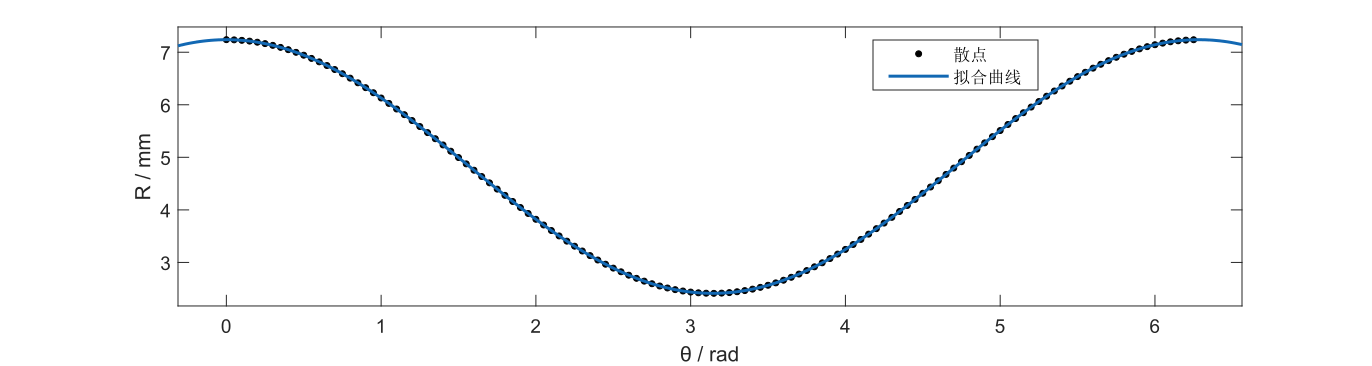
\includegraphics[width=.8\textwidth]{R_THETA.png}
	\caption{极径与极角关系图}
\end{figure}

液体的压强与密度的关系无简单的解析式,弹性模量一般是通过试验来确定的,因此直接选择用相关性最高的指数函数进行拟合得到式1, 拟合结果如图\ref{EP}. 
\begin{equation}
    E(P) = 1495e^{0.0039P} ,\quad \rm{R}^2 = 0.9955 \label{E} 
\end{equation}

\begin{figure}[htbp]
	\centering
	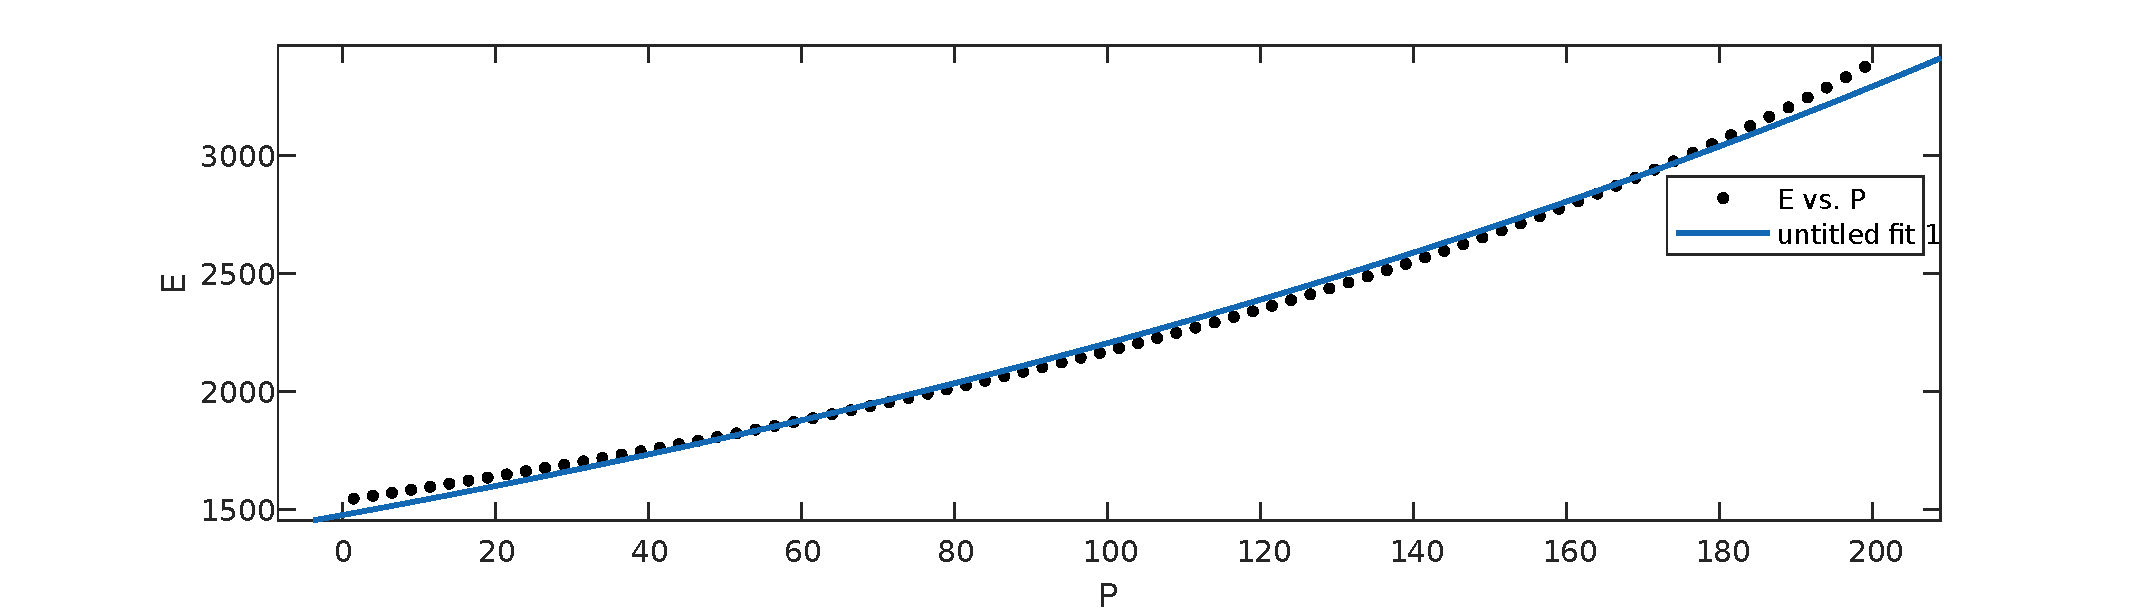
\includegraphics[width=.8\textwidth]{E_P.pdf}
    \caption{弹性模量与压强关系图}
    \label{EP}
\end{figure}

我们观测到针阀运动曲线的两端为S型曲线,S型曲线可以使用logistic回归进行拟合,便用此公式对针阀上升与下降过程进行分别的拟合,得到一个分段的函数

$$d_1 = \hua{
    \f{2.225}{1+537.9e^{-19.3t}}, &\quad t\in[0,0.45),&\quad \rm{R}^2=0.9996\\
    2,&\quad t\in[0.45,2),&\quad \rm{R}^2=1\\
    \f{2.267}{1+456.4e^{18.63(t-2.45)}}, &\quad t\in[2,2.45),&\quad \rm{R}^2=0.9997\\
    0,&\quad t\in[2.45, 100),&\quad \rm{R}^2=1
}$$

\begin{figure}[htbp]
	\centering
	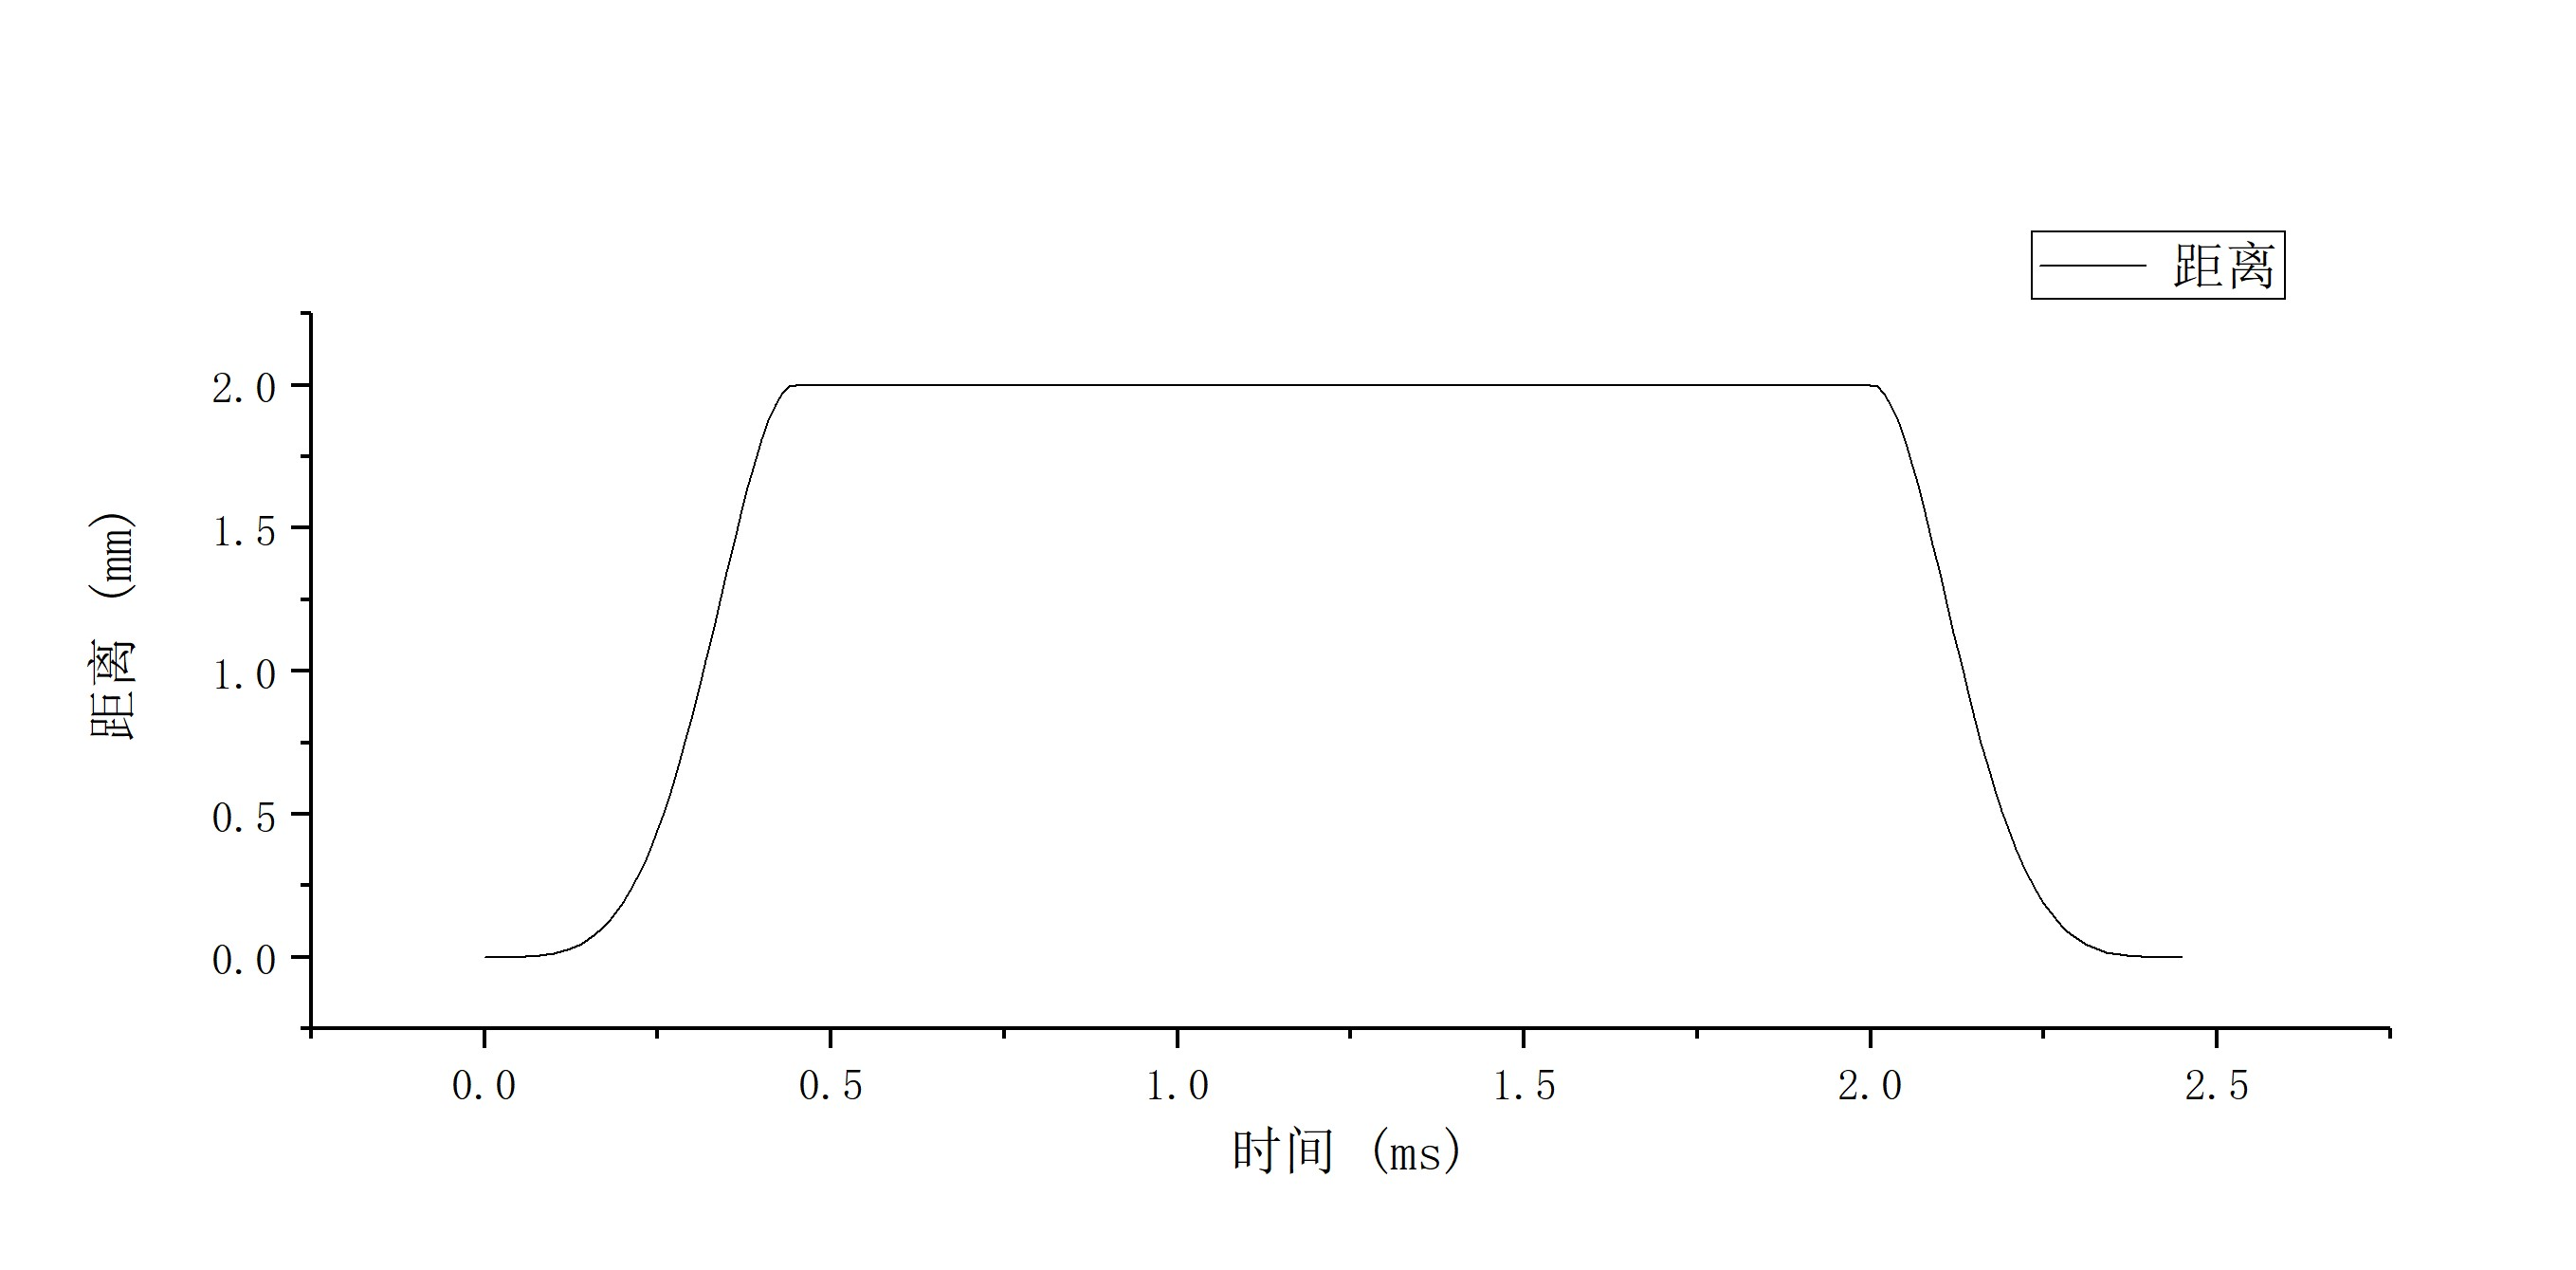
\includegraphics[width=.7\textwidth]{quan.jpg}
	\caption{针阀运动曲线}
\end{figure}
\subsection{问题一分析}
问题一共分两个小问. 

对于第一个小问, 高压油管内压力始终在100 MPa上下浮动. 对问题初步分析可以发现, 单次泵入, 喷出的燃油质量比油管内燃油质量低3个数量级. 因此忽略每次泵入、喷出燃油后油管内部的压力变化是合理的. 进行这样的假设后, 泵入流量$Q = CA\sqrt{\frac{2\Delta P}{\rho}} = 15.547\ \text{mm}^3/\text{ms}$将是一个恒定值. 又由于每次喷出的燃油体积$V_{out} = 440\text{ mm}^3$已知. 于是每秒需要泵入燃油的时间为$t_{s} = \frac{440\text{ mm}^3}{Q} = 28.3013\text{ ms}$. 为了让压力尽量稳定, 需要多次少量泵入燃油, 即使每次泵入燃油的间隔时间均为10 ms. 考虑这个条件之后, 设每次泵油时间为$t$, 便可写出1000 ms内喷油次数
$$N = \frac{1000}{t+10}=\frac{t_s}{t}$$
根据该方程即可得到每10 ms泵入一次油, 每次泵入燃油的时间:
$$\boxed{t = 0.29\text{ ms}}$$ 

对于第二个小问, 可以分解为油管内压力在规定时间内逐渐从100 MPa增加到150 MPa的过程一和使油管内压力保持在150 MPa的过程二. 

\begin{figure}[htbp]
    \centering
    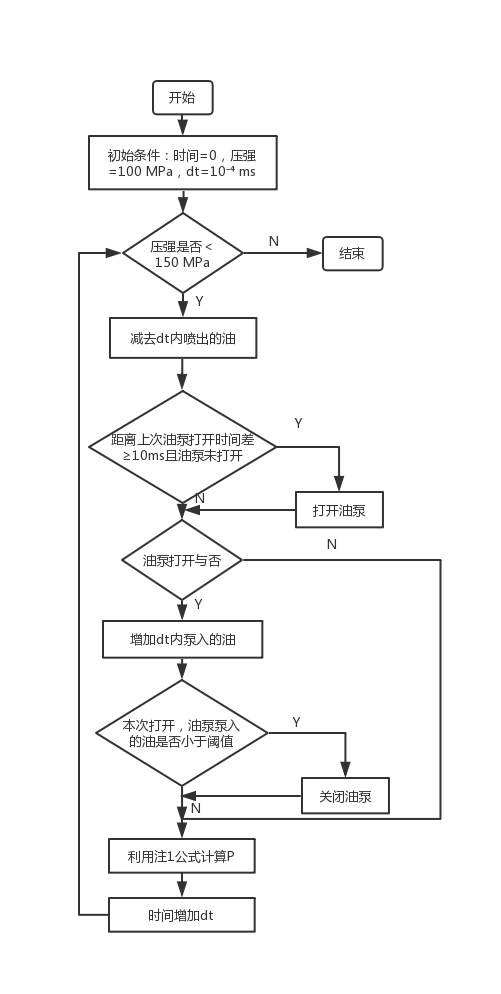
\includegraphics[width = 0.5\linewidth]{q1.jpg}
    \caption{问题一第二小问过程一流程图: 设定初值后, 开始按照$dt = 10^{-4}\ ms$逐渐增加时间$t$进行循环, 循环进行条件为压强小于$150\ MPa$, 在循环内, 先计算$dt$内喷出的油, 再判断此时是否需要打开阀门, 如果阀门已经打开, 则计算$dt$内泵入的油, 并判断此时是否需要关闭阀门. 结束后, 输出停止循环, 即得到$150\ MPa$需要的时间. }
    \label{121}
\end{figure}

对于过程一, 随着油管内压力逐渐增高, 泵入油的速率会逐渐降低, 但喷出油的速率保持不变. 为了保持油管内压力上升速率稳定, 应保持每次泵入的油量不变, 这会使每次开启泵的时间逐渐增加. 通过调节每次泵入的油的质量$m_B$的大小可以改变油管内压强的增加速度, 进而改变压强到达$150\ MPa$的时间. 实际计算中采用时间迭代的方法, , 计算泵入和喷出两个过程中每一个$\rm{d}t$内油量的微小变化. 其计算过程如图\ref{121}所示. 10000 ms内压强逐渐增加到150 MPa的过程如图\ref{12}所示.
\begin{figure}[htbp]
	\centering
	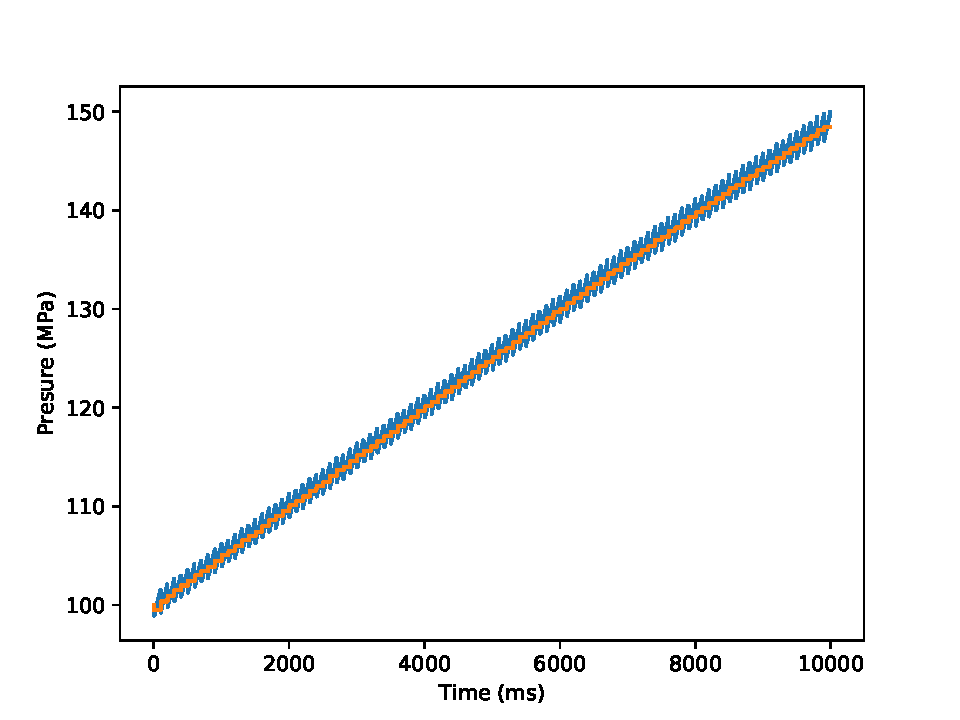
\includegraphics[width=.6\textwidth]{10000.pdf}
    \caption{第一题第二小问过程一: 10000 ms内压强逐渐增加到150 MPa的过程. 蓝线: 油管内压强, 橙线: 去除小范围波动后压强上升情况}
    \label{12}
\end{figure}

最终将得到不同时间达到150 MPa所需的每次泵入的油的质量$m_B$: 
\begin{center}
\begin{tabular}{|r|l|}
    \hline
    2 s & $m_B=$7.31 mg\\ 
    5 s & $m_B=$5.04 mg\\
    10 s & $m_B=$4.31 mg\\
    \hline
\end{tabular}
\end{center}



对于过程二, 此时问题简化为稳恒压力下泵入油策略, 将第一小问内部压强从100 MPa改变为150 MPa, 再将此时的密度替换为150 MPa下的密度即可. 

计算密度可利用注1中的公式
$$\ar{
    \d P \x \frac{E(P)}{\rho}\d \rho\\
    \f{\d P}{E(P)} \x \d(\ln\rho)
}$$
代入数据处理中得到的式\ref{E}:
$$E(P) = 1495e^{0.0039P}$$
积分并代入条件$\rho$ = 0.85 $\textup{mg}\cdot\rm{mm}^{-3}$, $ P = 100$ MPa可以得到
\begin{equation}
\rho = \f{1}{20.02}e^{-\f{1}{5.831}e^{-0.0039P}}  \label{rho}
\end{equation}
当$P =$150 MPa, 密度$\rho =$0.868 $\textup{mg}\cdot\rm{mm}^{-3}$时, 
每10 ms泵入一次油, 利用与第一小问相同的计算方法, 可得在150 MPa时每次泵油的时间为: 
$$\boxed{t = 0.75\ \rm{ms}}$$


\subsection{问题二分析}
对于问题二, 由于油管内压力始终在100 MPa上下小范围波动, 近似地认为油管内压力不变, 这个近似可以将泵油和喷油两个过程解耦合, 从而可以分开考虑这两个过程. 

\begin{figure}[htbp]
    \centering
    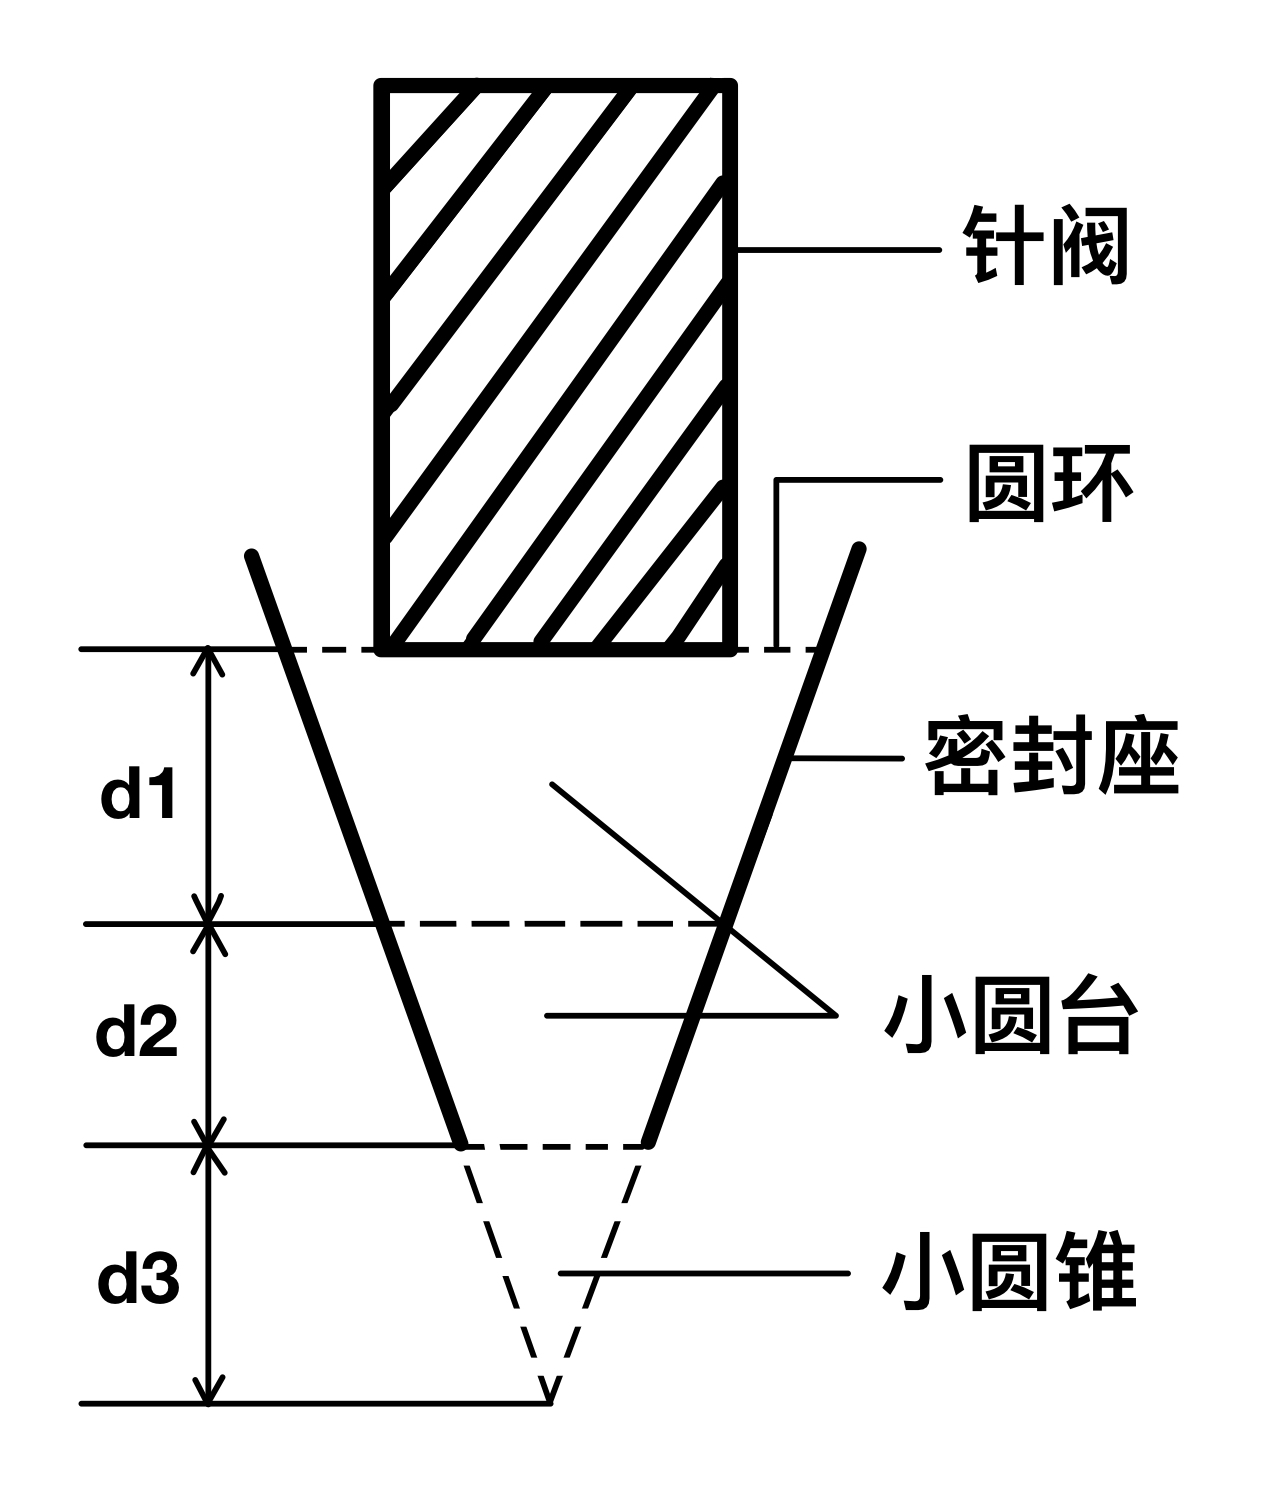
\includegraphics[width=0.2\textwidth]{penzui.jpg} 
    \caption{喷油嘴形状示意图: 将油从油管内进入小圆台内和从小圆台内进入外部环境看作两个出油过程}
    \label{penzui}
\end{figure}

对于喷油的过程, 喷油量的变化是固定的. 喷油嘴的形状如图\ref{penzui}所示. 将油从油管内穿过针阀底部和密封座形成的圆环进入圆台内, 和从圆台内穿过喷孔进入环境看做两个出油过程. 计算过程如图\ref{bout}所示. 在实际计算中发现, 几乎个$\d t$内喷入圆台的燃油都可以立刻从圆台完全喷出. 图\ref{bout2}展示了喷出的油的总质量随时间变化. 

\begin{figure}[htbp]
    \centering
    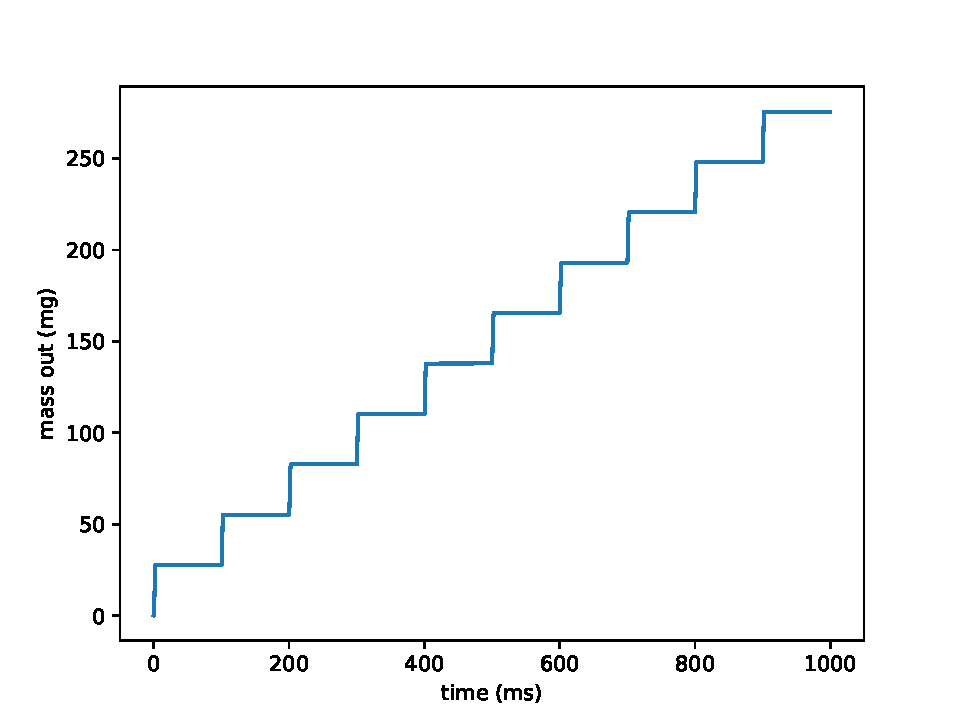
\includegraphics[width=0.5\textwidth]{bout2.pdf} 
    \caption{泵出的油的总质量随时间变化}
    \label{bout2}
\end{figure}

\begin{figure}[htbp]
    \centering
    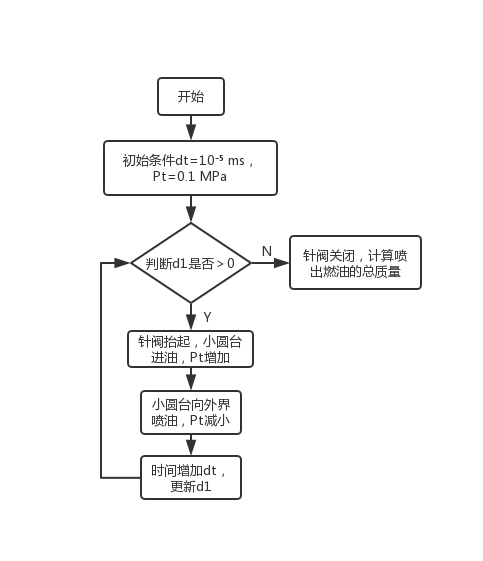
\includegraphics[width=0.6\textwidth]{bout.jpg} 
    \caption{喷油嘴形状示意图: 将油从油管内进入圆台内和从圆台内进入环境看做两个出油过程}
    \label{bout}
\end{figure}

对于泵油过程, 可以通过改变凸轮旋转的角速度来改变泵油的周期和每次泵油的油量. 可以将泵油过程分解成两种情况, 即油泵压力小于100 MPa不会向外泵油的情况和压力大于100 MPa会向油管泵油的情况. 

假设开始时油泵在下止点, 即极径最小的位置,油泵内将充满压强为0.5 MPa的低压燃油, 随着柱塞向上运动压缩燃油, 直到在$\theta = 0.515\ \rm{rad}$时燃油密度达到100 MPa对应的0.85 $\rm mg/mm^3$. 图\ref{bin1}展示了在刚开始时油泵内压力较低时油泵内压强随角度变化. 图\ref{bin}展示了当$\omega =0.3\ \rm{rad}$时油泵内压强随时间变化. 

\begin{figure}[htbp]
    \centering
    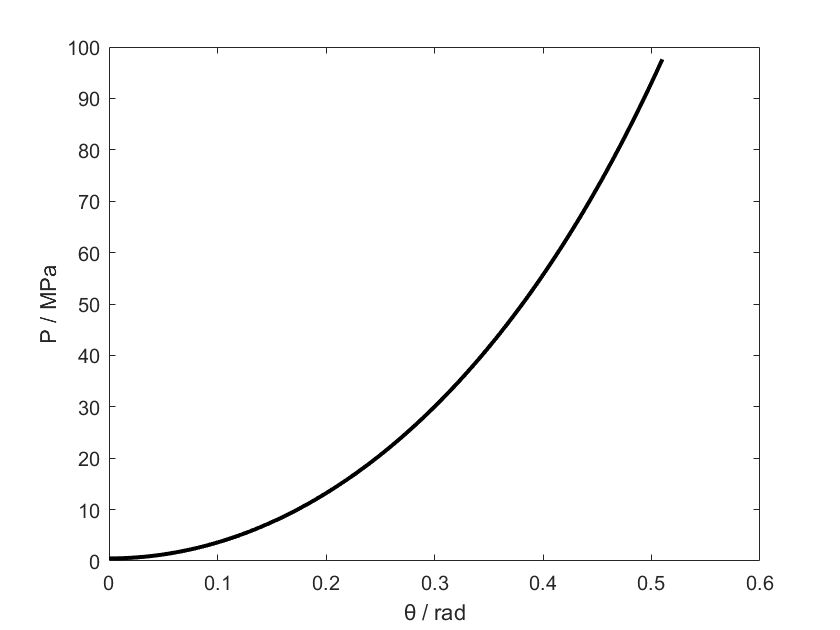
\includegraphics[width=0.6\textwidth]{THETA_P.png} 
    \caption{油泵内压强随时间变化}
    \label{bin1}
\end{figure}


\begin{figure}[htbp]
    \centering
    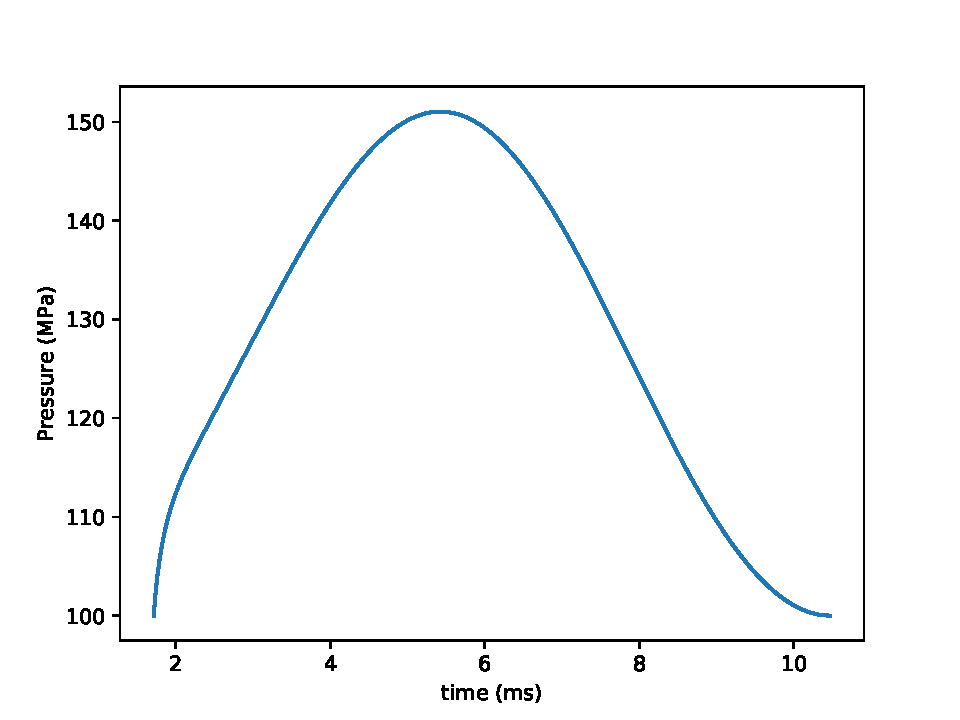
\includegraphics[width=0.6\textwidth]{bin_omega_0_3.pdf} 
    \caption{油泵内压强随时间变化}
    \label{bin}
\end{figure}


\subsection{问题三分析}

\section{模型评价与改进}
\subsection{模型的优点}
(1)在模型建立过程中,合理使用解耦合进行简化计算,模型创新性好。

(2)

(3)问题三采用变步长多次枚举法遍历求得,高压油管内压强稳定性得到显著提升。
\subsection{模型的缺点}
(1)求解压强稳定的最佳策略时,忽略了压强的微小波动,具有一定的局限性。

(2)查阅文献时发现,高压油管内是否是单相液质尚未有统一的定论,为了模型的简便,本文未考虑双相可能会带来的微小扰动。


\newpage
%参考文献
\begin{thebibliography}{9}%宽度9
 \bibitem{1} 殷子嘉.高压油管中燃油压力波传递速度的研究[J].上海交通大学学报,1992(01):47-51.
\end{thebibliography}

\newpage
%附录
\begin{appendices}
\section{排队算法--matlab 源程序}
\begin{lstlisting}[language=matlab]
kk=2;[mdd,ndd]=size(dd);
while ~isempty(V)
[tmpd,j]=min(W(i,V));tmpj=V(j);
for k=2:ndd
[tmp1,jj]=min(dd(1,k)+W(dd(2,k),V));
tmp2=V(jj);tt(k-1,:)=[tmp1,tmp2,jj];
end
tmp=[tmpd,tmpj,j;tt];[tmp3,tmp4]=min(tmp(:,1));
if tmp3==tmpd, ss(1:2,kk)=[i;tmp(tmp4,2)];
else,tmp5=find(ss(:,tmp4)~=0);tmp6=length(tmp5);
if dd(2,tmp4)==ss(tmp6,tmp4)
ss(1:tmp6+1,kk)=[ss(tmp5,tmp4);tmp(tmp4,2)];
else, ss(1:3,kk)=[i;dd(2,tmp4);tmp(tmp4,2)];
end;end
dd=[dd,[tmp3;tmp(tmp4,2)]];V(tmp(tmp4,3))=[];
[mdd,ndd]=size(dd);kk=kk+1;
end; S=ss; D=dd(1,:);
 \end{lstlisting}
 \section{规划解决程序--lingo源代码}
\begin{lstlisting}[language=c]
kk=2;
[mdd,ndd]=size(dd);
while ~isempty(V)
    [tmpd,j]=min(W(i,V));tmpj=V(j);
for k=2:ndd
    [tmp1,jj]=min(dd(1,k)+W(dd(2,k),V));
    tmp2=V(jj);tt(k-1,:)=[tmp1,tmp2,jj];
end
    tmp=[tmpd,tmpj,j;tt];[tmp3,tmp4]=min(tmp(:,1));
if tmp3==tmpd, ss(1:2,kk)=[i;tmp(tmp4,2)];
else,tmp5=find(ss(:,tmp4)~=0);tmp6=length(tmp5);
if dd(2,tmp4)==ss(tmp6,tmp4)
    ss(1:tmp6+1,kk)=[ss(tmp5,tmp4);tmp(tmp4,2)];
else, ss(1:3,kk)=[i;dd(2,tmp4);tmp(tmp4,2)];
end;
end
    dd=[dd,[tmp3;tmp(tmp4,2)]];V(tmp(tmp4,3))=[];
    [mdd,ndd]=size(dd);
    kk=kk+1;
end;
S=ss;
D=dd(1,:);
 \end{lstlisting}
\end{appendices}

\end{document} 